\chapter{Method}
\label{cha:method}

% In this chapter, the method is described in a way which shows how the
% work was actually carried out. The description must be precise and
% well thought through. Consider the scientific term
% replicability. Replicability means that someone reading a scientific
% report should be able to follow the method description and then carry
% out the same study and check whether the results obtained are
% similar. Achieving replicability is not always relevant, but precision
% and clarity is.
% 
% Sometimes the work is separated into different parts, e.g.  pre-study,
% implementation and evaluation. In such cases it is recommended that
% the method chapter is structured accordingly with suitable named
% sub-headings.

In this chapter, the method used is described.
Section \ref{sec:problem} formalizes the problem solved.
Section \ref{sec:environment} details the environment used to evaluate solutions.
Section \ref{sec:baseline} describes the baseline learning method.
Section \ref{sec:approach} describes the approach used to solve the problem with a learning agent.
Section \ref{sec:experiments} describes the experiments conducted to answer research questions \ref{itm:rq2} and \ref{itm:rq3}.

\section{Problem Statement}
\label{sec:problem}

% and problem formulation

% environment: discrete grid
% observation: subset of grid, equals attention
% action: transform subset of grid, trigger is binary decision telling whether target is found, or whether it should be checked for thoroughly?
% reward: used to achieve correct trigger in few actions

Formally, the searched environment contains a scene with a set of targets.
The scene is described by a Euclidean space.
In the scene, there are \(N\) targets, each described by a subspace.
At any given time the agent observes a subspace of the scene, which we call the view.
This observation is given in the form of an image.
Through a finite set of actions, the agent can transform its view.
With a final trigger action, the agent can indicate that there is a target in the view.
The goal of the agent is to bring all targets into the view and indicate that they have been found.
This is to be done with a minimal number of actions.
This corresponds to changing the field of perception.

We denote the task by \(\langle \mathcal{M}, \mathcal{T}_0 \rangle\), where \(\mathcal{M}\) is a POMDP and \(\mathcal{T}_0\) is the probability distribution on the initial states.

Furthermore, we make the assumption that the agent initially has access to its position.
With this, it can keep track of which regions are and have been in view before.

% "Learning to optimize" has some good formulation tips
% explains that policy search is intractable
% Also uses a decaying step size, could be interesting for us as well
% (although we have multiple targets...)

\section{Environment}
\label{sec:environment}

% overview
To train an test an agent for the problem, we use three environments of varying difficulty.
In each environment there is a scene with a background of distractors and a foreground of targets.
The scenes are drawn from some unknown distribution.
The background and foreground are assumed to be correlated.
This means that by looking at the background, an agent should sometimes be able to deduce a suitable action.
All scenes are assumed to be static in that the actions of the agent do not affect their appearance.

% observations, actions and rewards
The scenes of each environment are discretized into a grid.
We use the same action space, reward signal for all environments.
\(\mathcal{A} = \lbrace \mathtt{UP}, \mathtt{DOWN}, \mathtt{LEFT}, \mathtt{RIGHT}, \mathtt{TRIGGER} \rbrace\)
\(\mathcal{R(s, a)} = \dots\).
The observation space always includes the currently visible region of the environment, an RGB image \(x_t \in \mathbb{R}^{3 \times W \times H}\).
% reward inspired by Tabu Search?
% for multiple targets, give reward for moving towards closest target
% when to stop with multiple targets? automatically when all are found?

% use R^n notation for everything, including distance

Early experiments show that rewards like \(r_t = -1\) that simply incentivize the agent to complete the episode as quickly as possible are too slow to train and converge towards bad policies.
% cite something
% reason about good inductive biases
% would be interesting to see if the supervised distance reward generalizes worse

To incentivize finding targets quickly, the reward signal is set to -1 for each time step.
Since viewing a window twice is redundant, such actions are punished by setting the reward to -2.
If the agent selects the trigger action when a target overlaps with the window, the reward is set to 5.
When all targets have been triggered, or when 1000 time steps have passed, the episode ends.

Averaged over all possible samples, the probability of targets should be uniform over the scene.
% to make comparison with exhaustive search fair

% environment 1: easy, understandable
The first environment is the simplest environment. 
The scene is a two-dimensional discrete Euclidean space.
The appearance of the scene is given by a 256x256 RGB image.
The agent observes a 64x64 sub-image at each time step.
In the image there are three Gaussian kernels with random positions.
The height of the kernel is indicated by a higher intensity in the blue channel.
Targets are 1x1 pixels in the red channel.
The locations of the targets are randomized weighted by the height of the Gaussian kernels.
This means that the more intense the blue channel, the higher the probability of a target.
The idea with this environment is to test that the method learns what we want it to learn.
It is easy to determine whether the agent acts well in this environment.
Our feeling is that this is something that previous similar works has not done. % cite

\begin{figure}
    \centering
    %% Creator: Matplotlib, PGF backend
%%
%% To include the figure in your LaTeX document, write
%%   \input{<filename>.pgf}
%%
%% Make sure the required packages are loaded in your preamble
%%   \usepackage{pgf}
%%
%% Also ensure that all the required font packages are loaded; for instance,
%% the lmodern package is sometimes necessary when using math font.
%%   \usepackage{lmodern}
%%
%% Figures using additional raster images can only be included by \input if
%% they are in the same directory as the main LaTeX file. For loading figures
%% from other directories you can use the `import` package
%%   \usepackage{import}
%%
%% and then include the figures with
%%   \import{<path to file>}{<filename>.pgf}
%%
%% Matplotlib used the following preamble
%%   \usepackage{fontspec}
%%   \setmainfont{DejaVuSerif.ttf}[Path=\detokenize{/home/oslund/.local/lib/python3.8/site-packages/matplotlib/mpl-data/fonts/ttf/}]
%%   \setsansfont{DejaVuSans.ttf}[Path=\detokenize{/home/oslund/.local/lib/python3.8/site-packages/matplotlib/mpl-data/fonts/ttf/}]
%%   \setmonofont{DejaVuSansMono.ttf}[Path=\detokenize{/home/oslund/.local/lib/python3.8/site-packages/matplotlib/mpl-data/fonts/ttf/}]
%%
\begingroup%
\makeatletter%
\begin{pgfpicture}%
\pgfpathrectangle{\pgfpointorigin}{\pgfqpoint{5.645496in}{4.234122in}}%
\pgfusepath{use as bounding box, clip}%
\begin{pgfscope}%
\pgfsetbuttcap%
\pgfsetmiterjoin%
\definecolor{currentfill}{rgb}{1.000000,1.000000,1.000000}%
\pgfsetfillcolor{currentfill}%
\pgfsetlinewidth{0.000000pt}%
\definecolor{currentstroke}{rgb}{1.000000,1.000000,1.000000}%
\pgfsetstrokecolor{currentstroke}%
\pgfsetdash{}{0pt}%
\pgfpathmoveto{\pgfqpoint{0.000000in}{0.000000in}}%
\pgfpathlineto{\pgfqpoint{5.645496in}{0.000000in}}%
\pgfpathlineto{\pgfqpoint{5.645496in}{4.234122in}}%
\pgfpathlineto{\pgfqpoint{0.000000in}{4.234122in}}%
\pgfpathlineto{\pgfqpoint{0.000000in}{0.000000in}}%
\pgfpathclose%
\pgfusepath{fill}%
\end{pgfscope}%
\begin{pgfscope}%
\pgfsetbuttcap%
\pgfsetmiterjoin%
\definecolor{currentfill}{rgb}{1.000000,1.000000,1.000000}%
\pgfsetfillcolor{currentfill}%
\pgfsetlinewidth{0.000000pt}%
\definecolor{currentstroke}{rgb}{0.000000,0.000000,0.000000}%
\pgfsetstrokecolor{currentstroke}%
\pgfsetstrokeopacity{0.000000}%
\pgfsetdash{}{0pt}%
\pgfpathmoveto{\pgfqpoint{0.705687in}{0.478947in}}%
\pgfpathlineto{\pgfqpoint{3.939574in}{0.478947in}}%
\pgfpathlineto{\pgfqpoint{3.939574in}{3.712834in}}%
\pgfpathlineto{\pgfqpoint{0.705687in}{3.712834in}}%
\pgfpathlineto{\pgfqpoint{0.705687in}{0.478947in}}%
\pgfpathclose%
\pgfusepath{fill}%
\end{pgfscope}%
\begin{pgfscope}%
\pgfpathrectangle{\pgfqpoint{0.705687in}{0.478947in}}{\pgfqpoint{3.233887in}{3.233887in}}%
\pgfusepath{clip}%
\pgfsys@transformshift{0.705687in}{0.478947in}%
\pgftext[left,bottom]{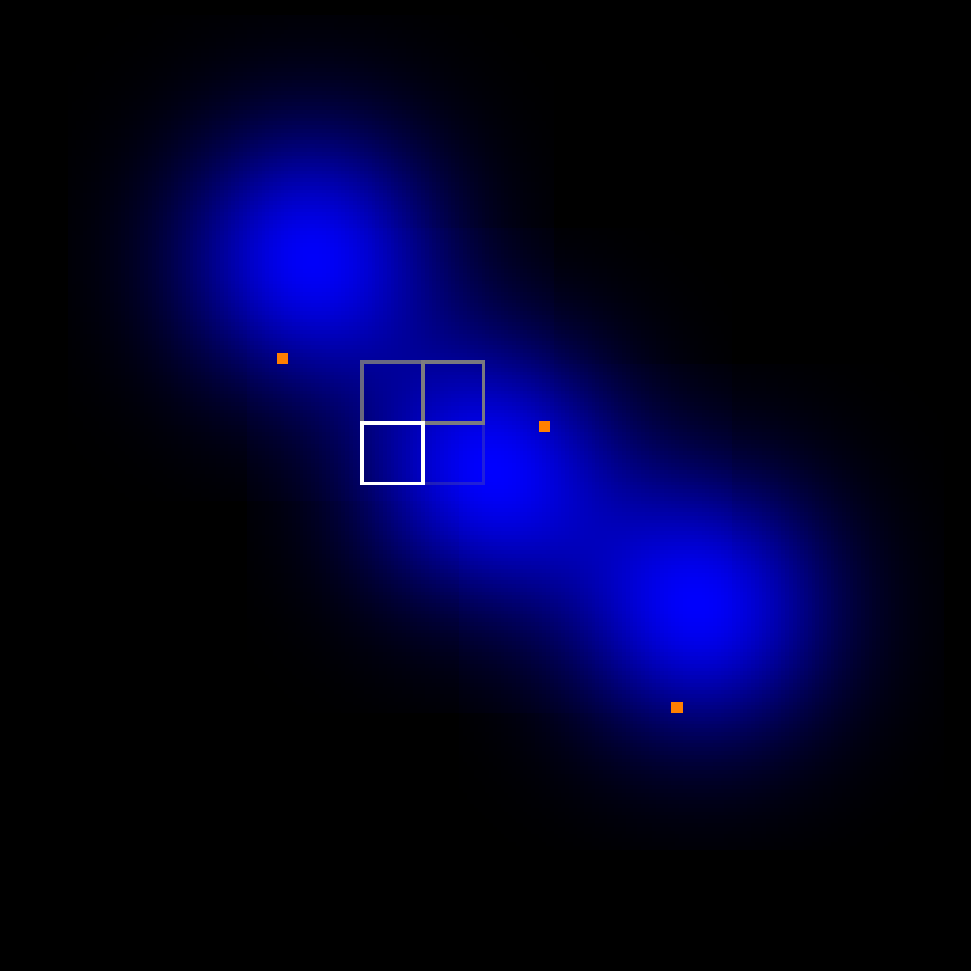
\includegraphics[interpolate=true,width=3.236667in,height=3.236667in]{gaussian-img0.png}}%
\end{pgfscope}%
\begin{pgfscope}%
\pgfpathrectangle{\pgfqpoint{0.705687in}{0.478947in}}{\pgfqpoint{3.233887in}{3.233887in}}%
\pgfusepath{clip}%
\pgfsetbuttcap%
\pgfsetmiterjoin%
\pgfsetlinewidth{0.752812pt}%
\definecolor{currentstroke}{rgb}{1.000000,0.000000,0.000000}%
\pgfsetstrokecolor{currentstroke}%
\pgfsetdash{{2.775000pt}{1.200000pt}}{0.000000pt}%
\pgfpathmoveto{\pgfqpoint{2.935301in}{1.543856in}}%
\pgfpathcurveto{\pgfqpoint{2.978183in}{1.543856in}}{\pgfqpoint{3.019314in}{1.526819in}}{\pgfqpoint{3.049636in}{1.496497in}}%
\pgfpathcurveto{\pgfqpoint{3.079958in}{1.466174in}}{\pgfqpoint{3.096995in}{1.425043in}}{\pgfqpoint{3.096995in}{1.382161in}}%
\pgfpathcurveto{\pgfqpoint{3.096995in}{1.339280in}}{\pgfqpoint{3.079958in}{1.298148in}}{\pgfqpoint{3.049636in}{1.267826in}}%
\pgfpathcurveto{\pgfqpoint{3.019314in}{1.237504in}}{\pgfqpoint{2.978183in}{1.220467in}}{\pgfqpoint{2.935301in}{1.220467in}}%
\pgfpathcurveto{\pgfqpoint{2.892419in}{1.220467in}}{\pgfqpoint{2.851288in}{1.237504in}}{\pgfqpoint{2.820966in}{1.267826in}}%
\pgfpathcurveto{\pgfqpoint{2.790644in}{1.298148in}}{\pgfqpoint{2.773606in}{1.339280in}}{\pgfqpoint{2.773606in}{1.382161in}}%
\pgfpathcurveto{\pgfqpoint{2.773606in}{1.425043in}}{\pgfqpoint{2.790644in}{1.466174in}}{\pgfqpoint{2.820966in}{1.496497in}}%
\pgfpathcurveto{\pgfqpoint{2.851288in}{1.526819in}}{\pgfqpoint{2.892419in}{1.543856in}}{\pgfqpoint{2.935301in}{1.543856in}}%
\pgfpathlineto{\pgfqpoint{2.935301in}{1.543856in}}%
\pgfpathclose%
\pgfusepath{stroke}%
\end{pgfscope}%
\begin{pgfscope}%
\pgfpathrectangle{\pgfqpoint{0.705687in}{0.478947in}}{\pgfqpoint{3.233887in}{3.233887in}}%
\pgfusepath{clip}%
\pgfsetbuttcap%
\pgfsetmiterjoin%
\pgfsetlinewidth{0.752812pt}%
\definecolor{currentstroke}{rgb}{1.000000,0.000000,0.000000}%
\pgfsetstrokecolor{currentstroke}%
\pgfsetdash{{2.775000pt}{1.200000pt}}{0.000000pt}%
\pgfpathmoveto{\pgfqpoint{1.621534in}{2.706034in}}%
\pgfpathcurveto{\pgfqpoint{1.664416in}{2.706034in}}{\pgfqpoint{1.705547in}{2.688997in}}{\pgfqpoint{1.735869in}{2.658675in}}%
\pgfpathcurveto{\pgfqpoint{1.766191in}{2.628353in}}{\pgfqpoint{1.783228in}{2.587221in}}{\pgfqpoint{1.783228in}{2.544340in}}%
\pgfpathcurveto{\pgfqpoint{1.783228in}{2.501458in}}{\pgfqpoint{1.766191in}{2.460327in}}{\pgfqpoint{1.735869in}{2.430004in}}%
\pgfpathcurveto{\pgfqpoint{1.705547in}{2.399682in}}{\pgfqpoint{1.664416in}{2.382645in}}{\pgfqpoint{1.621534in}{2.382645in}}%
\pgfpathcurveto{\pgfqpoint{1.578652in}{2.382645in}}{\pgfqpoint{1.537521in}{2.399682in}}{\pgfqpoint{1.507199in}{2.430004in}}%
\pgfpathcurveto{\pgfqpoint{1.476877in}{2.460327in}}{\pgfqpoint{1.459840in}{2.501458in}}{\pgfqpoint{1.459840in}{2.544340in}}%
\pgfpathcurveto{\pgfqpoint{1.459840in}{2.587221in}}{\pgfqpoint{1.476877in}{2.628353in}}{\pgfqpoint{1.507199in}{2.658675in}}%
\pgfpathcurveto{\pgfqpoint{1.537521in}{2.688997in}}{\pgfqpoint{1.578652in}{2.706034in}}{\pgfqpoint{1.621534in}{2.706034in}}%
\pgfpathlineto{\pgfqpoint{1.621534in}{2.706034in}}%
\pgfpathclose%
\pgfusepath{stroke}%
\end{pgfscope}%
\begin{pgfscope}%
\pgfpathrectangle{\pgfqpoint{0.705687in}{0.478947in}}{\pgfqpoint{3.233887in}{3.233887in}}%
\pgfusepath{clip}%
\pgfsetbuttcap%
\pgfsetmiterjoin%
\pgfsetlinewidth{0.752812pt}%
\definecolor{currentstroke}{rgb}{1.000000,0.000000,0.000000}%
\pgfsetstrokecolor{currentstroke}%
\pgfsetdash{{2.775000pt}{1.200000pt}}{0.000000pt}%
\pgfpathmoveto{\pgfqpoint{2.493168in}{2.478651in}}%
\pgfpathcurveto{\pgfqpoint{2.536050in}{2.478651in}}{\pgfqpoint{2.577181in}{2.461614in}}{\pgfqpoint{2.607503in}{2.431292in}}%
\pgfpathcurveto{\pgfqpoint{2.637825in}{2.400970in}}{\pgfqpoint{2.654862in}{2.359839in}}{\pgfqpoint{2.654862in}{2.316957in}}%
\pgfpathcurveto{\pgfqpoint{2.654862in}{2.274075in}}{\pgfqpoint{2.637825in}{2.232944in}}{\pgfqpoint{2.607503in}{2.202622in}}%
\pgfpathcurveto{\pgfqpoint{2.577181in}{2.172300in}}{\pgfqpoint{2.536050in}{2.155263in}}{\pgfqpoint{2.493168in}{2.155263in}}%
\pgfpathcurveto{\pgfqpoint{2.450286in}{2.155263in}}{\pgfqpoint{2.409155in}{2.172300in}}{\pgfqpoint{2.378833in}{2.202622in}}%
\pgfpathcurveto{\pgfqpoint{2.348511in}{2.232944in}}{\pgfqpoint{2.331473in}{2.274075in}}{\pgfqpoint{2.331473in}{2.316957in}}%
\pgfpathcurveto{\pgfqpoint{2.331473in}{2.359839in}}{\pgfqpoint{2.348511in}{2.400970in}}{\pgfqpoint{2.378833in}{2.431292in}}%
\pgfpathcurveto{\pgfqpoint{2.409155in}{2.461614in}}{\pgfqpoint{2.450286in}{2.478651in}}{\pgfqpoint{2.493168in}{2.478651in}}%
\pgfpathlineto{\pgfqpoint{2.493168in}{2.478651in}}%
\pgfpathclose%
\pgfusepath{stroke}%
\end{pgfscope}%
\begin{pgfscope}%
\pgfsetbuttcap%
\pgfsetroundjoin%
\definecolor{currentfill}{rgb}{0.000000,0.000000,0.000000}%
\pgfsetfillcolor{currentfill}%
\pgfsetlinewidth{0.803000pt}%
\definecolor{currentstroke}{rgb}{0.000000,0.000000,0.000000}%
\pgfsetstrokecolor{currentstroke}%
\pgfsetdash{}{0pt}%
\pgfsys@defobject{currentmarker}{\pgfqpoint{0.000000in}{-0.048611in}}{\pgfqpoint{0.000000in}{0.000000in}}{%
\pgfpathmoveto{\pgfqpoint{0.000000in}{0.000000in}}%
\pgfpathlineto{\pgfqpoint{0.000000in}{-0.048611in}}%
\pgfusepath{stroke,fill}%
}%
\begin{pgfscope}%
\pgfsys@transformshift{0.712003in}{0.478947in}%
\pgfsys@useobject{currentmarker}{}%
\end{pgfscope}%
\end{pgfscope}%
\begin{pgfscope}%
\definecolor{textcolor}{rgb}{0.000000,0.000000,0.000000}%
\pgfsetstrokecolor{textcolor}%
\pgfsetfillcolor{textcolor}%
\pgftext[x=0.712003in,y=0.381724in,,top]{\color{textcolor}\rmfamily\fontsize{8.000000}{9.600000}\selectfont \(\displaystyle {0}\)}%
\end{pgfscope}%
\begin{pgfscope}%
\pgfsetbuttcap%
\pgfsetroundjoin%
\definecolor{currentfill}{rgb}{0.000000,0.000000,0.000000}%
\pgfsetfillcolor{currentfill}%
\pgfsetlinewidth{0.803000pt}%
\definecolor{currentstroke}{rgb}{0.000000,0.000000,0.000000}%
\pgfsetstrokecolor{currentstroke}%
\pgfsetdash{}{0pt}%
\pgfsys@defobject{currentmarker}{\pgfqpoint{0.000000in}{-0.048611in}}{\pgfqpoint{0.000000in}{0.000000in}}{%
\pgfpathmoveto{\pgfqpoint{0.000000in}{0.000000in}}%
\pgfpathlineto{\pgfqpoint{0.000000in}{-0.048611in}}%
\pgfusepath{stroke,fill}%
}%
\begin{pgfscope}%
\pgfsys@transformshift{1.343622in}{0.478947in}%
\pgfsys@useobject{currentmarker}{}%
\end{pgfscope}%
\end{pgfscope}%
\begin{pgfscope}%
\definecolor{textcolor}{rgb}{0.000000,0.000000,0.000000}%
\pgfsetstrokecolor{textcolor}%
\pgfsetfillcolor{textcolor}%
\pgftext[x=1.343622in,y=0.381724in,,top]{\color{textcolor}\rmfamily\fontsize{8.000000}{9.600000}\selectfont \(\displaystyle {50}\)}%
\end{pgfscope}%
\begin{pgfscope}%
\pgfsetbuttcap%
\pgfsetroundjoin%
\definecolor{currentfill}{rgb}{0.000000,0.000000,0.000000}%
\pgfsetfillcolor{currentfill}%
\pgfsetlinewidth{0.803000pt}%
\definecolor{currentstroke}{rgb}{0.000000,0.000000,0.000000}%
\pgfsetstrokecolor{currentstroke}%
\pgfsetdash{}{0pt}%
\pgfsys@defobject{currentmarker}{\pgfqpoint{0.000000in}{-0.048611in}}{\pgfqpoint{0.000000in}{0.000000in}}{%
\pgfpathmoveto{\pgfqpoint{0.000000in}{0.000000in}}%
\pgfpathlineto{\pgfqpoint{0.000000in}{-0.048611in}}%
\pgfusepath{stroke,fill}%
}%
\begin{pgfscope}%
\pgfsys@transformshift{1.975240in}{0.478947in}%
\pgfsys@useobject{currentmarker}{}%
\end{pgfscope}%
\end{pgfscope}%
\begin{pgfscope}%
\definecolor{textcolor}{rgb}{0.000000,0.000000,0.000000}%
\pgfsetstrokecolor{textcolor}%
\pgfsetfillcolor{textcolor}%
\pgftext[x=1.975240in,y=0.381724in,,top]{\color{textcolor}\rmfamily\fontsize{8.000000}{9.600000}\selectfont \(\displaystyle {100}\)}%
\end{pgfscope}%
\begin{pgfscope}%
\pgfsetbuttcap%
\pgfsetroundjoin%
\definecolor{currentfill}{rgb}{0.000000,0.000000,0.000000}%
\pgfsetfillcolor{currentfill}%
\pgfsetlinewidth{0.803000pt}%
\definecolor{currentstroke}{rgb}{0.000000,0.000000,0.000000}%
\pgfsetstrokecolor{currentstroke}%
\pgfsetdash{}{0pt}%
\pgfsys@defobject{currentmarker}{\pgfqpoint{0.000000in}{-0.048611in}}{\pgfqpoint{0.000000in}{0.000000in}}{%
\pgfpathmoveto{\pgfqpoint{0.000000in}{0.000000in}}%
\pgfpathlineto{\pgfqpoint{0.000000in}{-0.048611in}}%
\pgfusepath{stroke,fill}%
}%
\begin{pgfscope}%
\pgfsys@transformshift{2.606859in}{0.478947in}%
\pgfsys@useobject{currentmarker}{}%
\end{pgfscope}%
\end{pgfscope}%
\begin{pgfscope}%
\definecolor{textcolor}{rgb}{0.000000,0.000000,0.000000}%
\pgfsetstrokecolor{textcolor}%
\pgfsetfillcolor{textcolor}%
\pgftext[x=2.606859in,y=0.381724in,,top]{\color{textcolor}\rmfamily\fontsize{8.000000}{9.600000}\selectfont \(\displaystyle {150}\)}%
\end{pgfscope}%
\begin{pgfscope}%
\pgfsetbuttcap%
\pgfsetroundjoin%
\definecolor{currentfill}{rgb}{0.000000,0.000000,0.000000}%
\pgfsetfillcolor{currentfill}%
\pgfsetlinewidth{0.803000pt}%
\definecolor{currentstroke}{rgb}{0.000000,0.000000,0.000000}%
\pgfsetstrokecolor{currentstroke}%
\pgfsetdash{}{0pt}%
\pgfsys@defobject{currentmarker}{\pgfqpoint{0.000000in}{-0.048611in}}{\pgfqpoint{0.000000in}{0.000000in}}{%
\pgfpathmoveto{\pgfqpoint{0.000000in}{0.000000in}}%
\pgfpathlineto{\pgfqpoint{0.000000in}{-0.048611in}}%
\pgfusepath{stroke,fill}%
}%
\begin{pgfscope}%
\pgfsys@transformshift{3.238478in}{0.478947in}%
\pgfsys@useobject{currentmarker}{}%
\end{pgfscope}%
\end{pgfscope}%
\begin{pgfscope}%
\definecolor{textcolor}{rgb}{0.000000,0.000000,0.000000}%
\pgfsetstrokecolor{textcolor}%
\pgfsetfillcolor{textcolor}%
\pgftext[x=3.238478in,y=0.381724in,,top]{\color{textcolor}\rmfamily\fontsize{8.000000}{9.600000}\selectfont \(\displaystyle {200}\)}%
\end{pgfscope}%
\begin{pgfscope}%
\pgfsetbuttcap%
\pgfsetroundjoin%
\definecolor{currentfill}{rgb}{0.000000,0.000000,0.000000}%
\pgfsetfillcolor{currentfill}%
\pgfsetlinewidth{0.803000pt}%
\definecolor{currentstroke}{rgb}{0.000000,0.000000,0.000000}%
\pgfsetstrokecolor{currentstroke}%
\pgfsetdash{}{0pt}%
\pgfsys@defobject{currentmarker}{\pgfqpoint{0.000000in}{-0.048611in}}{\pgfqpoint{0.000000in}{0.000000in}}{%
\pgfpathmoveto{\pgfqpoint{0.000000in}{0.000000in}}%
\pgfpathlineto{\pgfqpoint{0.000000in}{-0.048611in}}%
\pgfusepath{stroke,fill}%
}%
\begin{pgfscope}%
\pgfsys@transformshift{3.870096in}{0.478947in}%
\pgfsys@useobject{currentmarker}{}%
\end{pgfscope}%
\end{pgfscope}%
\begin{pgfscope}%
\definecolor{textcolor}{rgb}{0.000000,0.000000,0.000000}%
\pgfsetstrokecolor{textcolor}%
\pgfsetfillcolor{textcolor}%
\pgftext[x=3.870096in,y=0.381724in,,top]{\color{textcolor}\rmfamily\fontsize{8.000000}{9.600000}\selectfont \(\displaystyle {250}\)}%
\end{pgfscope}%
\begin{pgfscope}%
\pgfsetbuttcap%
\pgfsetroundjoin%
\definecolor{currentfill}{rgb}{0.000000,0.000000,0.000000}%
\pgfsetfillcolor{currentfill}%
\pgfsetlinewidth{0.803000pt}%
\definecolor{currentstroke}{rgb}{0.000000,0.000000,0.000000}%
\pgfsetstrokecolor{currentstroke}%
\pgfsetdash{}{0pt}%
\pgfsys@defobject{currentmarker}{\pgfqpoint{-0.048611in}{0.000000in}}{\pgfqpoint{-0.000000in}{0.000000in}}{%
\pgfpathmoveto{\pgfqpoint{-0.000000in}{0.000000in}}%
\pgfpathlineto{\pgfqpoint{-0.048611in}{0.000000in}}%
\pgfusepath{stroke,fill}%
}%
\begin{pgfscope}%
\pgfsys@transformshift{0.705687in}{3.706518in}%
\pgfsys@useobject{currentmarker}{}%
\end{pgfscope}%
\end{pgfscope}%
\begin{pgfscope}%
\definecolor{textcolor}{rgb}{0.000000,0.000000,0.000000}%
\pgfsetstrokecolor{textcolor}%
\pgfsetfillcolor{textcolor}%
\pgftext[x=0.549436in, y=3.664309in, left, base]{\color{textcolor}\rmfamily\fontsize{8.000000}{9.600000}\selectfont \(\displaystyle {0}\)}%
\end{pgfscope}%
\begin{pgfscope}%
\pgfsetbuttcap%
\pgfsetroundjoin%
\definecolor{currentfill}{rgb}{0.000000,0.000000,0.000000}%
\pgfsetfillcolor{currentfill}%
\pgfsetlinewidth{0.803000pt}%
\definecolor{currentstroke}{rgb}{0.000000,0.000000,0.000000}%
\pgfsetstrokecolor{currentstroke}%
\pgfsetdash{}{0pt}%
\pgfsys@defobject{currentmarker}{\pgfqpoint{-0.048611in}{0.000000in}}{\pgfqpoint{-0.000000in}{0.000000in}}{%
\pgfpathmoveto{\pgfqpoint{-0.000000in}{0.000000in}}%
\pgfpathlineto{\pgfqpoint{-0.048611in}{0.000000in}}%
\pgfusepath{stroke,fill}%
}%
\begin{pgfscope}%
\pgfsys@transformshift{0.705687in}{3.074899in}%
\pgfsys@useobject{currentmarker}{}%
\end{pgfscope}%
\end{pgfscope}%
\begin{pgfscope}%
\definecolor{textcolor}{rgb}{0.000000,0.000000,0.000000}%
\pgfsetstrokecolor{textcolor}%
\pgfsetfillcolor{textcolor}%
\pgftext[x=0.490408in, y=3.032690in, left, base]{\color{textcolor}\rmfamily\fontsize{8.000000}{9.600000}\selectfont \(\displaystyle {50}\)}%
\end{pgfscope}%
\begin{pgfscope}%
\pgfsetbuttcap%
\pgfsetroundjoin%
\definecolor{currentfill}{rgb}{0.000000,0.000000,0.000000}%
\pgfsetfillcolor{currentfill}%
\pgfsetlinewidth{0.803000pt}%
\definecolor{currentstroke}{rgb}{0.000000,0.000000,0.000000}%
\pgfsetstrokecolor{currentstroke}%
\pgfsetdash{}{0pt}%
\pgfsys@defobject{currentmarker}{\pgfqpoint{-0.048611in}{0.000000in}}{\pgfqpoint{-0.000000in}{0.000000in}}{%
\pgfpathmoveto{\pgfqpoint{-0.000000in}{0.000000in}}%
\pgfpathlineto{\pgfqpoint{-0.048611in}{0.000000in}}%
\pgfusepath{stroke,fill}%
}%
\begin{pgfscope}%
\pgfsys@transformshift{0.705687in}{2.443281in}%
\pgfsys@useobject{currentmarker}{}%
\end{pgfscope}%
\end{pgfscope}%
\begin{pgfscope}%
\definecolor{textcolor}{rgb}{0.000000,0.000000,0.000000}%
\pgfsetstrokecolor{textcolor}%
\pgfsetfillcolor{textcolor}%
\pgftext[x=0.431379in, y=2.401071in, left, base]{\color{textcolor}\rmfamily\fontsize{8.000000}{9.600000}\selectfont \(\displaystyle {100}\)}%
\end{pgfscope}%
\begin{pgfscope}%
\pgfsetbuttcap%
\pgfsetroundjoin%
\definecolor{currentfill}{rgb}{0.000000,0.000000,0.000000}%
\pgfsetfillcolor{currentfill}%
\pgfsetlinewidth{0.803000pt}%
\definecolor{currentstroke}{rgb}{0.000000,0.000000,0.000000}%
\pgfsetstrokecolor{currentstroke}%
\pgfsetdash{}{0pt}%
\pgfsys@defobject{currentmarker}{\pgfqpoint{-0.048611in}{0.000000in}}{\pgfqpoint{-0.000000in}{0.000000in}}{%
\pgfpathmoveto{\pgfqpoint{-0.000000in}{0.000000in}}%
\pgfpathlineto{\pgfqpoint{-0.048611in}{0.000000in}}%
\pgfusepath{stroke,fill}%
}%
\begin{pgfscope}%
\pgfsys@transformshift{0.705687in}{1.811662in}%
\pgfsys@useobject{currentmarker}{}%
\end{pgfscope}%
\end{pgfscope}%
\begin{pgfscope}%
\definecolor{textcolor}{rgb}{0.000000,0.000000,0.000000}%
\pgfsetstrokecolor{textcolor}%
\pgfsetfillcolor{textcolor}%
\pgftext[x=0.431379in, y=1.769453in, left, base]{\color{textcolor}\rmfamily\fontsize{8.000000}{9.600000}\selectfont \(\displaystyle {150}\)}%
\end{pgfscope}%
\begin{pgfscope}%
\pgfsetbuttcap%
\pgfsetroundjoin%
\definecolor{currentfill}{rgb}{0.000000,0.000000,0.000000}%
\pgfsetfillcolor{currentfill}%
\pgfsetlinewidth{0.803000pt}%
\definecolor{currentstroke}{rgb}{0.000000,0.000000,0.000000}%
\pgfsetstrokecolor{currentstroke}%
\pgfsetdash{}{0pt}%
\pgfsys@defobject{currentmarker}{\pgfqpoint{-0.048611in}{0.000000in}}{\pgfqpoint{-0.000000in}{0.000000in}}{%
\pgfpathmoveto{\pgfqpoint{-0.000000in}{0.000000in}}%
\pgfpathlineto{\pgfqpoint{-0.048611in}{0.000000in}}%
\pgfusepath{stroke,fill}%
}%
\begin{pgfscope}%
\pgfsys@transformshift{0.705687in}{1.180043in}%
\pgfsys@useobject{currentmarker}{}%
\end{pgfscope}%
\end{pgfscope}%
\begin{pgfscope}%
\definecolor{textcolor}{rgb}{0.000000,0.000000,0.000000}%
\pgfsetstrokecolor{textcolor}%
\pgfsetfillcolor{textcolor}%
\pgftext[x=0.431379in, y=1.137834in, left, base]{\color{textcolor}\rmfamily\fontsize{8.000000}{9.600000}\selectfont \(\displaystyle {200}\)}%
\end{pgfscope}%
\begin{pgfscope}%
\pgfsetbuttcap%
\pgfsetroundjoin%
\definecolor{currentfill}{rgb}{0.000000,0.000000,0.000000}%
\pgfsetfillcolor{currentfill}%
\pgfsetlinewidth{0.803000pt}%
\definecolor{currentstroke}{rgb}{0.000000,0.000000,0.000000}%
\pgfsetstrokecolor{currentstroke}%
\pgfsetdash{}{0pt}%
\pgfsys@defobject{currentmarker}{\pgfqpoint{-0.048611in}{0.000000in}}{\pgfqpoint{-0.000000in}{0.000000in}}{%
\pgfpathmoveto{\pgfqpoint{-0.000000in}{0.000000in}}%
\pgfpathlineto{\pgfqpoint{-0.048611in}{0.000000in}}%
\pgfusepath{stroke,fill}%
}%
\begin{pgfscope}%
\pgfsys@transformshift{0.705687in}{0.548425in}%
\pgfsys@useobject{currentmarker}{}%
\end{pgfscope}%
\end{pgfscope}%
\begin{pgfscope}%
\definecolor{textcolor}{rgb}{0.000000,0.000000,0.000000}%
\pgfsetstrokecolor{textcolor}%
\pgfsetfillcolor{textcolor}%
\pgftext[x=0.431379in, y=0.506216in, left, base]{\color{textcolor}\rmfamily\fontsize{8.000000}{9.600000}\selectfont \(\displaystyle {250}\)}%
\end{pgfscope}%
\begin{pgfscope}%
\pgfsetrectcap%
\pgfsetmiterjoin%
\pgfsetlinewidth{0.803000pt}%
\definecolor{currentstroke}{rgb}{0.000000,0.000000,0.000000}%
\pgfsetstrokecolor{currentstroke}%
\pgfsetdash{}{0pt}%
\pgfpathmoveto{\pgfqpoint{0.705687in}{0.478947in}}%
\pgfpathlineto{\pgfqpoint{0.705687in}{3.712834in}}%
\pgfusepath{stroke}%
\end{pgfscope}%
\begin{pgfscope}%
\pgfsetrectcap%
\pgfsetmiterjoin%
\pgfsetlinewidth{0.803000pt}%
\definecolor{currentstroke}{rgb}{0.000000,0.000000,0.000000}%
\pgfsetstrokecolor{currentstroke}%
\pgfsetdash{}{0pt}%
\pgfpathmoveto{\pgfqpoint{3.939574in}{0.478947in}}%
\pgfpathlineto{\pgfqpoint{3.939574in}{3.712834in}}%
\pgfusepath{stroke}%
\end{pgfscope}%
\begin{pgfscope}%
\pgfsetrectcap%
\pgfsetmiterjoin%
\pgfsetlinewidth{0.803000pt}%
\definecolor{currentstroke}{rgb}{0.000000,0.000000,0.000000}%
\pgfsetstrokecolor{currentstroke}%
\pgfsetdash{}{0pt}%
\pgfpathmoveto{\pgfqpoint{0.705687in}{0.478947in}}%
\pgfpathlineto{\pgfqpoint{3.939574in}{0.478947in}}%
\pgfusepath{stroke}%
\end{pgfscope}%
\begin{pgfscope}%
\pgfsetrectcap%
\pgfsetmiterjoin%
\pgfsetlinewidth{0.803000pt}%
\definecolor{currentstroke}{rgb}{0.000000,0.000000,0.000000}%
\pgfsetstrokecolor{currentstroke}%
\pgfsetdash{}{0pt}%
\pgfpathmoveto{\pgfqpoint{0.705687in}{3.712834in}}%
\pgfpathlineto{\pgfqpoint{3.939574in}{3.712834in}}%
\pgfusepath{stroke}%
\end{pgfscope}%
\begin{pgfscope}%
\pgfpathrectangle{\pgfqpoint{4.129803in}{2.771004in}}{\pgfqpoint{0.951143in}{0.951143in}}%
\pgfusepath{clip}%
\pgfsys@transformshift{4.129803in}{2.771004in}%
\pgftext[left,bottom]{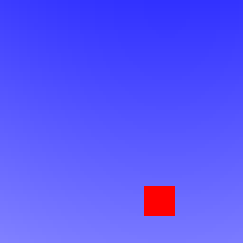
\includegraphics[interpolate=true,width=0.953333in,height=0.953333in]{gaussian-img1.png}}%
\end{pgfscope}%
\begin{pgfscope}%
\pgfpathrectangle{\pgfqpoint{4.129803in}{1.620319in}}{\pgfqpoint{0.951143in}{0.951143in}}%
\pgfusepath{clip}%
\pgfsys@transformshift{4.129803in}{1.620319in}%
\pgftext[left,bottom]{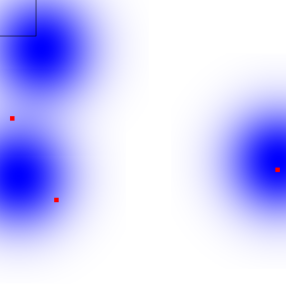
\includegraphics[interpolate=true,width=0.953333in,height=0.953333in]{gaussian-img2.png}}%
\end{pgfscope}%
\begin{pgfscope}%
\pgfpathrectangle{\pgfqpoint{4.129803in}{0.469634in}}{\pgfqpoint{0.951143in}{0.951143in}}%
\pgfusepath{clip}%
\pgfsys@transformshift{4.129803in}{0.469634in}%
\pgftext[left,bottom]{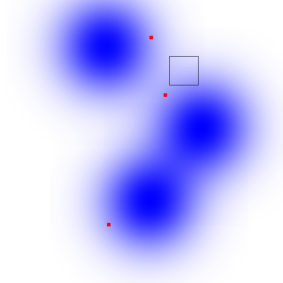
\includegraphics[interpolate=true,width=0.953333in,height=0.953333in]{gaussian-img3.png}}%
\end{pgfscope}%
\end{pgfpicture}%
\makeatother%
\endgroup%

    \label{fig:gaussian}
    %\vspace*{-1cm}
    \caption{Four samples of the first environment. There are three gaussian kernels in the environment, whose height is visualized with the blue channel. There are three targets in the environment, whose location is sampled from the distribution defined by the sum of the three gaussian kernels.}
\end{figure}

% environment 2: medium, procedural and configurable
The second environment is intended to look like realistic terrain.
The environment has a two-dimensional scene whose appearance is given by a 512x512 image.
Gradient noise is generated and used as a height map.
The height map determines the color of the terrain.
The height also correlates to the probability of targets.
Specifically, targets are located between shores and mountain bases.
This environment simulates a UAV search-and-rescue scenario.

\begin{figure}
    \centering
    %% Creator: Matplotlib, PGF backend
%%
%% To include the figure in your LaTeX document, write
%%   \input{<filename>.pgf}
%%
%% Make sure the required packages are loaded in your preamble
%%   \usepackage{pgf}
%%
%% Also ensure that all the required font packages are loaded; for instance,
%% the lmodern package is sometimes necessary when using math font.
%%   \usepackage{lmodern}
%%
%% Figures using additional raster images can only be included by \input if
%% they are in the same directory as the main LaTeX file. For loading figures
%% from other directories you can use the `import` package
%%   \usepackage{import}
%%
%% and then include the figures with
%%   \import{<path to file>}{<filename>.pgf}
%%
%% Matplotlib used the following preamble
%%   \usepackage{fontspec}
%%   \setmainfont{DejaVuSerif.ttf}[Path=\detokenize{/usr/lib/python3.10/site-packages/matplotlib/mpl-data/fonts/ttf/}]
%%   \setsansfont{DejaVuSans.ttf}[Path=\detokenize{/usr/lib/python3.10/site-packages/matplotlib/mpl-data/fonts/ttf/}]
%%   \setmonofont{DejaVuSansMono.ttf}[Path=\detokenize{/usr/lib/python3.10/site-packages/matplotlib/mpl-data/fonts/ttf/}]
%%
\begingroup%
\makeatletter%
\begin{pgfpicture}%
\pgfpathrectangle{\pgfpointorigin}{\pgfqpoint{5.645496in}{4.234122in}}%
\pgfusepath{use as bounding box, clip}%
\begin{pgfscope}%
\pgfsetbuttcap%
\pgfsetmiterjoin%
\definecolor{currentfill}{rgb}{1.000000,1.000000,1.000000}%
\pgfsetfillcolor{currentfill}%
\pgfsetlinewidth{0.000000pt}%
\definecolor{currentstroke}{rgb}{1.000000,1.000000,1.000000}%
\pgfsetstrokecolor{currentstroke}%
\pgfsetdash{}{0pt}%
\pgfpathmoveto{\pgfqpoint{0.000000in}{0.000000in}}%
\pgfpathlineto{\pgfqpoint{5.645496in}{0.000000in}}%
\pgfpathlineto{\pgfqpoint{5.645496in}{4.234122in}}%
\pgfpathlineto{\pgfqpoint{0.000000in}{4.234122in}}%
\pgfpathlineto{\pgfqpoint{0.000000in}{0.000000in}}%
\pgfpathclose%
\pgfusepath{fill}%
\end{pgfscope}%
\begin{pgfscope}%
\pgfsetbuttcap%
\pgfsetmiterjoin%
\definecolor{currentfill}{rgb}{1.000000,1.000000,1.000000}%
\pgfsetfillcolor{currentfill}%
\pgfsetlinewidth{0.000000pt}%
\definecolor{currentstroke}{rgb}{0.000000,0.000000,0.000000}%
\pgfsetstrokecolor{currentstroke}%
\pgfsetstrokeopacity{0.000000}%
\pgfsetdash{}{0pt}%
\pgfpathmoveto{\pgfqpoint{0.705687in}{0.478947in}}%
\pgfpathlineto{\pgfqpoint{3.939574in}{0.478947in}}%
\pgfpathlineto{\pgfqpoint{3.939574in}{3.712834in}}%
\pgfpathlineto{\pgfqpoint{0.705687in}{3.712834in}}%
\pgfpathlineto{\pgfqpoint{0.705687in}{0.478947in}}%
\pgfpathclose%
\pgfusepath{fill}%
\end{pgfscope}%
\begin{pgfscope}%
\pgfpathrectangle{\pgfqpoint{0.705687in}{0.478947in}}{\pgfqpoint{3.233887in}{3.233887in}}%
\pgfusepath{clip}%
\pgfsys@transformshift{0.705687in}{0.478947in}%
\pgftext[left,bottom]{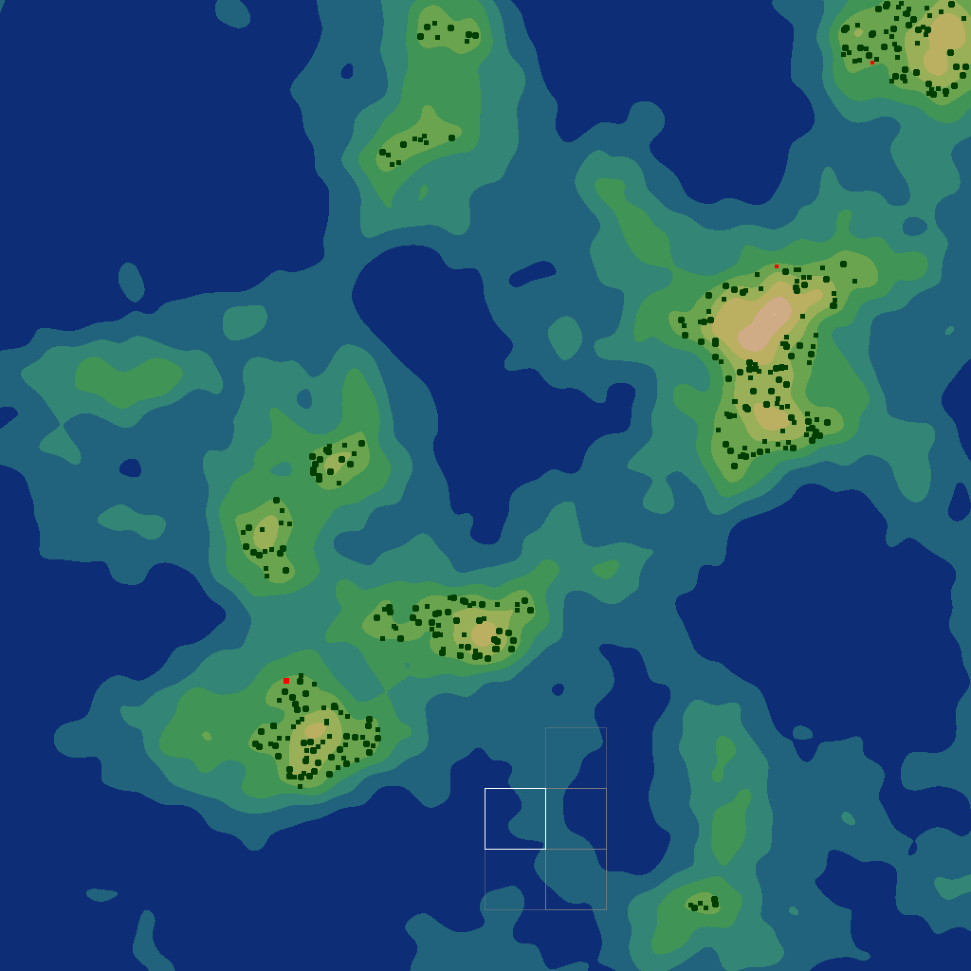
\includegraphics[interpolate=true,width=3.236667in,height=3.236667in]{terrain-img0.png}}%
\end{pgfscope}%
\begin{pgfscope}%
\pgfsetbuttcap%
\pgfsetroundjoin%
\definecolor{currentfill}{rgb}{0.000000,0.000000,0.000000}%
\pgfsetfillcolor{currentfill}%
\pgfsetlinewidth{0.803000pt}%
\definecolor{currentstroke}{rgb}{0.000000,0.000000,0.000000}%
\pgfsetstrokecolor{currentstroke}%
\pgfsetdash{}{0pt}%
\pgfsys@defobject{currentmarker}{\pgfqpoint{0.000000in}{-0.048611in}}{\pgfqpoint{0.000000in}{0.000000in}}{%
\pgfpathmoveto{\pgfqpoint{0.000000in}{0.000000in}}%
\pgfpathlineto{\pgfqpoint{0.000000in}{-0.048611in}}%
\pgfusepath{stroke,fill}%
}%
\begin{pgfscope}%
\pgfsys@transformshift{0.707266in}{0.478947in}%
\pgfsys@useobject{currentmarker}{}%
\end{pgfscope}%
\end{pgfscope}%
\begin{pgfscope}%
\definecolor{textcolor}{rgb}{0.000000,0.000000,0.000000}%
\pgfsetstrokecolor{textcolor}%
\pgfsetfillcolor{textcolor}%
\pgftext[x=0.707266in,y=0.381724in,,top]{\color{textcolor}\rmfamily\fontsize{8.000000}{9.600000}\selectfont \(\displaystyle {0}\)}%
\end{pgfscope}%
\begin{pgfscope}%
\pgfsetbuttcap%
\pgfsetroundjoin%
\definecolor{currentfill}{rgb}{0.000000,0.000000,0.000000}%
\pgfsetfillcolor{currentfill}%
\pgfsetlinewidth{0.803000pt}%
\definecolor{currentstroke}{rgb}{0.000000,0.000000,0.000000}%
\pgfsetstrokecolor{currentstroke}%
\pgfsetdash{}{0pt}%
\pgfsys@defobject{currentmarker}{\pgfqpoint{0.000000in}{-0.048611in}}{\pgfqpoint{0.000000in}{0.000000in}}{%
\pgfpathmoveto{\pgfqpoint{0.000000in}{0.000000in}}%
\pgfpathlineto{\pgfqpoint{0.000000in}{-0.048611in}}%
\pgfusepath{stroke,fill}%
}%
\begin{pgfscope}%
\pgfsys@transformshift{3.937995in}{0.478947in}%
\pgfsys@useobject{currentmarker}{}%
\end{pgfscope}%
\end{pgfscope}%
\begin{pgfscope}%
\definecolor{textcolor}{rgb}{0.000000,0.000000,0.000000}%
\pgfsetstrokecolor{textcolor}%
\pgfsetfillcolor{textcolor}%
\pgftext[x=3.937995in,y=0.381724in,,top]{\color{textcolor}\rmfamily\fontsize{8.000000}{9.600000}\selectfont \(\displaystyle {1023}\)}%
\end{pgfscope}%
\begin{pgfscope}%
\pgfsetbuttcap%
\pgfsetroundjoin%
\definecolor{currentfill}{rgb}{0.000000,0.000000,0.000000}%
\pgfsetfillcolor{currentfill}%
\pgfsetlinewidth{0.803000pt}%
\definecolor{currentstroke}{rgb}{0.000000,0.000000,0.000000}%
\pgfsetstrokecolor{currentstroke}%
\pgfsetdash{}{0pt}%
\pgfsys@defobject{currentmarker}{\pgfqpoint{-0.048611in}{0.000000in}}{\pgfqpoint{-0.000000in}{0.000000in}}{%
\pgfpathmoveto{\pgfqpoint{-0.000000in}{0.000000in}}%
\pgfpathlineto{\pgfqpoint{-0.048611in}{0.000000in}}%
\pgfusepath{stroke,fill}%
}%
\begin{pgfscope}%
\pgfsys@transformshift{0.705687in}{3.711255in}%
\pgfsys@useobject{currentmarker}{}%
\end{pgfscope}%
\end{pgfscope}%
\begin{pgfscope}%
\definecolor{textcolor}{rgb}{0.000000,0.000000,0.000000}%
\pgfsetstrokecolor{textcolor}%
\pgfsetfillcolor{textcolor}%
\pgftext[x=0.549436in, y=3.669046in, left, base]{\color{textcolor}\rmfamily\fontsize{8.000000}{9.600000}\selectfont \(\displaystyle {0}\)}%
\end{pgfscope}%
\begin{pgfscope}%
\pgfsetbuttcap%
\pgfsetroundjoin%
\definecolor{currentfill}{rgb}{0.000000,0.000000,0.000000}%
\pgfsetfillcolor{currentfill}%
\pgfsetlinewidth{0.803000pt}%
\definecolor{currentstroke}{rgb}{0.000000,0.000000,0.000000}%
\pgfsetstrokecolor{currentstroke}%
\pgfsetdash{}{0pt}%
\pgfsys@defobject{currentmarker}{\pgfqpoint{-0.048611in}{0.000000in}}{\pgfqpoint{-0.000000in}{0.000000in}}{%
\pgfpathmoveto{\pgfqpoint{-0.000000in}{0.000000in}}%
\pgfpathlineto{\pgfqpoint{-0.048611in}{0.000000in}}%
\pgfusepath{stroke,fill}%
}%
\begin{pgfscope}%
\pgfsys@transformshift{0.705687in}{0.480526in}%
\pgfsys@useobject{currentmarker}{}%
\end{pgfscope}%
\end{pgfscope}%
\begin{pgfscope}%
\definecolor{textcolor}{rgb}{0.000000,0.000000,0.000000}%
\pgfsetstrokecolor{textcolor}%
\pgfsetfillcolor{textcolor}%
\pgftext[x=0.372350in, y=0.438317in, left, base]{\color{textcolor}\rmfamily\fontsize{8.000000}{9.600000}\selectfont \(\displaystyle {1023}\)}%
\end{pgfscope}%
\begin{pgfscope}%
\pgfsetrectcap%
\pgfsetmiterjoin%
\pgfsetlinewidth{0.803000pt}%
\definecolor{currentstroke}{rgb}{0.000000,0.000000,0.000000}%
\pgfsetstrokecolor{currentstroke}%
\pgfsetdash{}{0pt}%
\pgfpathmoveto{\pgfqpoint{0.705687in}{0.478947in}}%
\pgfpathlineto{\pgfqpoint{0.705687in}{3.712834in}}%
\pgfusepath{stroke}%
\end{pgfscope}%
\begin{pgfscope}%
\pgfsetrectcap%
\pgfsetmiterjoin%
\pgfsetlinewidth{0.803000pt}%
\definecolor{currentstroke}{rgb}{0.000000,0.000000,0.000000}%
\pgfsetstrokecolor{currentstroke}%
\pgfsetdash{}{0pt}%
\pgfpathmoveto{\pgfqpoint{3.939574in}{0.478947in}}%
\pgfpathlineto{\pgfqpoint{3.939574in}{3.712834in}}%
\pgfusepath{stroke}%
\end{pgfscope}%
\begin{pgfscope}%
\pgfsetrectcap%
\pgfsetmiterjoin%
\pgfsetlinewidth{0.803000pt}%
\definecolor{currentstroke}{rgb}{0.000000,0.000000,0.000000}%
\pgfsetstrokecolor{currentstroke}%
\pgfsetdash{}{0pt}%
\pgfpathmoveto{\pgfqpoint{0.705687in}{0.478947in}}%
\pgfpathlineto{\pgfqpoint{3.939574in}{0.478947in}}%
\pgfusepath{stroke}%
\end{pgfscope}%
\begin{pgfscope}%
\pgfsetrectcap%
\pgfsetmiterjoin%
\pgfsetlinewidth{0.803000pt}%
\definecolor{currentstroke}{rgb}{0.000000,0.000000,0.000000}%
\pgfsetstrokecolor{currentstroke}%
\pgfsetdash{}{0pt}%
\pgfpathmoveto{\pgfqpoint{0.705687in}{3.712834in}}%
\pgfpathlineto{\pgfqpoint{3.939574in}{3.712834in}}%
\pgfusepath{stroke}%
\end{pgfscope}%
\begin{pgfscope}%
\pgfpathrectangle{\pgfqpoint{0.705687in}{0.478947in}}{\pgfqpoint{3.233887in}{3.233887in}}%
\pgfusepath{clip}%
\pgfsetbuttcap%
\pgfsetmiterjoin%
\pgfsetlinewidth{1.003750pt}%
\definecolor{currentstroke}{rgb}{0.000000,0.000000,0.000000}%
\pgfsetstrokecolor{currentstroke}%
\pgfsetstrokeopacity{0.500000}%
\pgfsetdash{}{0pt}%
\pgfpathmoveto{\pgfqpoint{1.515738in}{2.094311in}}%
\pgfpathlineto{\pgfqpoint{1.717856in}{2.094311in}}%
\pgfpathlineto{\pgfqpoint{1.717856in}{1.892193in}}%
\pgfpathlineto{\pgfqpoint{1.515738in}{1.892193in}}%
\pgfpathlineto{\pgfqpoint{1.515738in}{2.094311in}}%
\pgfpathclose%
\pgfusepath{stroke}%
\end{pgfscope}%
\begin{pgfscope}%
\pgfsetroundcap%
\pgfsetroundjoin%
\pgfsetlinewidth{1.003750pt}%
\definecolor{currentstroke}{rgb}{0.000000,0.000000,0.000000}%
\pgfsetstrokecolor{currentstroke}%
\pgfsetstrokeopacity{0.500000}%
\pgfsetdash{}{0pt}%
\pgfpathmoveto{\pgfqpoint{1.029076in}{1.610807in}}%
\pgfpathquadraticcurveto{\pgfqpoint{1.272407in}{1.852559in}}{\pgfqpoint{1.515738in}{2.094311in}}%
\pgfusepath{stroke}%
\end{pgfscope}%
\begin{pgfscope}%
\pgfsetroundcap%
\pgfsetroundjoin%
\pgfsetlinewidth{1.003750pt}%
\definecolor{currentstroke}{rgb}{0.000000,0.000000,0.000000}%
\pgfsetstrokecolor{currentstroke}%
\pgfsetstrokeopacity{0.500000}%
\pgfsetdash{}{0pt}%
\pgfpathmoveto{\pgfqpoint{1.837548in}{1.610807in}}%
\pgfpathquadraticcurveto{\pgfqpoint{1.777702in}{1.852559in}}{\pgfqpoint{1.717856in}{2.094311in}}%
\pgfusepath{stroke}%
\end{pgfscope}%
\begin{pgfscope}%
\pgfsetbuttcap%
\pgfsetmiterjoin%
\definecolor{currentfill}{rgb}{1.000000,1.000000,1.000000}%
\pgfsetfillcolor{currentfill}%
\pgfsetlinewidth{0.000000pt}%
\definecolor{currentstroke}{rgb}{0.000000,0.000000,0.000000}%
\pgfsetstrokecolor{currentstroke}%
\pgfsetstrokeopacity{0.000000}%
\pgfsetdash{}{0pt}%
\pgfpathmoveto{\pgfqpoint{1.029076in}{0.802335in}}%
\pgfpathlineto{\pgfqpoint{1.837548in}{0.802335in}}%
\pgfpathlineto{\pgfqpoint{1.837548in}{1.610807in}}%
\pgfpathlineto{\pgfqpoint{1.029076in}{1.610807in}}%
\pgfpathlineto{\pgfqpoint{1.029076in}{0.802335in}}%
\pgfpathclose%
\pgfusepath{fill}%
\end{pgfscope}%
\begin{pgfscope}%
\pgfpathrectangle{\pgfqpoint{1.029076in}{0.802335in}}{\pgfqpoint{0.808472in}{0.808472in}}%
\pgfusepath{clip}%
\pgfsys@transformshift{1.029076in}{0.802335in}%
\pgftext[left,bottom]{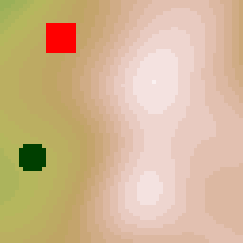
\includegraphics[interpolate=true,width=0.810000in,height=0.810000in]{terrain-img1.png}}%
\end{pgfscope}%
\begin{pgfscope}%
\pgfsetbuttcap%
\pgfsetroundjoin%
\definecolor{currentfill}{rgb}{0.000000,0.000000,0.000000}%
\pgfsetfillcolor{currentfill}%
\pgfsetlinewidth{0.803000pt}%
\definecolor{currentstroke}{rgb}{0.000000,0.000000,0.000000}%
\pgfsetstrokecolor{currentstroke}%
\pgfsetdash{}{0pt}%
\pgfsys@defobject{currentmarker}{\pgfqpoint{0.000000in}{-0.048611in}}{\pgfqpoint{0.000000in}{0.000000in}}{%
\pgfpathmoveto{\pgfqpoint{0.000000in}{0.000000in}}%
\pgfpathlineto{\pgfqpoint{0.000000in}{-0.048611in}}%
\pgfusepath{stroke,fill}%
}%
\begin{pgfscope}%
\pgfsys@transformshift{1.035392in}{0.802335in}%
\pgfsys@useobject{currentmarker}{}%
\end{pgfscope}%
\end{pgfscope}%
\begin{pgfscope}%
\definecolor{textcolor}{rgb}{0.000000,0.000000,0.000000}%
\pgfsetstrokecolor{textcolor}%
\pgfsetfillcolor{textcolor}%
\pgftext[x=1.035392in,y=0.705113in,,top]{\color{textcolor}\rmfamily\fontsize{8.000000}{9.600000}\selectfont \(\displaystyle {0}\)}%
\end{pgfscope}%
\begin{pgfscope}%
\pgfsetbuttcap%
\pgfsetroundjoin%
\definecolor{currentfill}{rgb}{0.000000,0.000000,0.000000}%
\pgfsetfillcolor{currentfill}%
\pgfsetlinewidth{0.803000pt}%
\definecolor{currentstroke}{rgb}{0.000000,0.000000,0.000000}%
\pgfsetstrokecolor{currentstroke}%
\pgfsetdash{}{0pt}%
\pgfsys@defobject{currentmarker}{\pgfqpoint{0.000000in}{-0.048611in}}{\pgfqpoint{0.000000in}{0.000000in}}{%
\pgfpathmoveto{\pgfqpoint{0.000000in}{0.000000in}}%
\pgfpathlineto{\pgfqpoint{0.000000in}{-0.048611in}}%
\pgfusepath{stroke,fill}%
}%
\begin{pgfscope}%
\pgfsys@transformshift{1.831231in}{0.802335in}%
\pgfsys@useobject{currentmarker}{}%
\end{pgfscope}%
\end{pgfscope}%
\begin{pgfscope}%
\definecolor{textcolor}{rgb}{0.000000,0.000000,0.000000}%
\pgfsetstrokecolor{textcolor}%
\pgfsetfillcolor{textcolor}%
\pgftext[x=1.831231in,y=0.705113in,,top]{\color{textcolor}\rmfamily\fontsize{8.000000}{9.600000}\selectfont \(\displaystyle {63}\)}%
\end{pgfscope}%
\begin{pgfscope}%
\pgfsetbuttcap%
\pgfsetroundjoin%
\definecolor{currentfill}{rgb}{0.000000,0.000000,0.000000}%
\pgfsetfillcolor{currentfill}%
\pgfsetlinewidth{0.803000pt}%
\definecolor{currentstroke}{rgb}{0.000000,0.000000,0.000000}%
\pgfsetstrokecolor{currentstroke}%
\pgfsetdash{}{0pt}%
\pgfsys@defobject{currentmarker}{\pgfqpoint{-0.048611in}{0.000000in}}{\pgfqpoint{-0.000000in}{0.000000in}}{%
\pgfpathmoveto{\pgfqpoint{-0.000000in}{0.000000in}}%
\pgfpathlineto{\pgfqpoint{-0.048611in}{0.000000in}}%
\pgfusepath{stroke,fill}%
}%
\begin{pgfscope}%
\pgfsys@transformshift{1.029076in}{1.604491in}%
\pgfsys@useobject{currentmarker}{}%
\end{pgfscope}%
\end{pgfscope}%
\begin{pgfscope}%
\definecolor{textcolor}{rgb}{0.000000,0.000000,0.000000}%
\pgfsetstrokecolor{textcolor}%
\pgfsetfillcolor{textcolor}%
\pgftext[x=0.872825in, y=1.562282in, left, base]{\color{textcolor}\rmfamily\fontsize{8.000000}{9.600000}\selectfont \(\displaystyle {0}\)}%
\end{pgfscope}%
\begin{pgfscope}%
\pgfsetbuttcap%
\pgfsetroundjoin%
\definecolor{currentfill}{rgb}{0.000000,0.000000,0.000000}%
\pgfsetfillcolor{currentfill}%
\pgfsetlinewidth{0.803000pt}%
\definecolor{currentstroke}{rgb}{0.000000,0.000000,0.000000}%
\pgfsetstrokecolor{currentstroke}%
\pgfsetdash{}{0pt}%
\pgfsys@defobject{currentmarker}{\pgfqpoint{-0.048611in}{0.000000in}}{\pgfqpoint{-0.000000in}{0.000000in}}{%
\pgfpathmoveto{\pgfqpoint{-0.000000in}{0.000000in}}%
\pgfpathlineto{\pgfqpoint{-0.048611in}{0.000000in}}%
\pgfusepath{stroke,fill}%
}%
\begin{pgfscope}%
\pgfsys@transformshift{1.029076in}{0.808652in}%
\pgfsys@useobject{currentmarker}{}%
\end{pgfscope}%
\end{pgfscope}%
\begin{pgfscope}%
\definecolor{textcolor}{rgb}{0.000000,0.000000,0.000000}%
\pgfsetstrokecolor{textcolor}%
\pgfsetfillcolor{textcolor}%
\pgftext[x=0.813796in, y=0.766442in, left, base]{\color{textcolor}\rmfamily\fontsize{8.000000}{9.600000}\selectfont \(\displaystyle {63}\)}%
\end{pgfscope}%
\begin{pgfscope}%
\pgfsetrectcap%
\pgfsetmiterjoin%
\pgfsetlinewidth{0.803000pt}%
\definecolor{currentstroke}{rgb}{0.000000,0.000000,0.000000}%
\pgfsetstrokecolor{currentstroke}%
\pgfsetdash{}{0pt}%
\pgfpathmoveto{\pgfqpoint{1.029076in}{0.802335in}}%
\pgfpathlineto{\pgfqpoint{1.029076in}{1.610807in}}%
\pgfusepath{stroke}%
\end{pgfscope}%
\begin{pgfscope}%
\pgfsetrectcap%
\pgfsetmiterjoin%
\pgfsetlinewidth{0.803000pt}%
\definecolor{currentstroke}{rgb}{0.000000,0.000000,0.000000}%
\pgfsetstrokecolor{currentstroke}%
\pgfsetdash{}{0pt}%
\pgfpathmoveto{\pgfqpoint{1.837548in}{0.802335in}}%
\pgfpathlineto{\pgfqpoint{1.837548in}{1.610807in}}%
\pgfusepath{stroke}%
\end{pgfscope}%
\begin{pgfscope}%
\pgfsetrectcap%
\pgfsetmiterjoin%
\pgfsetlinewidth{0.803000pt}%
\definecolor{currentstroke}{rgb}{0.000000,0.000000,0.000000}%
\pgfsetstrokecolor{currentstroke}%
\pgfsetdash{}{0pt}%
\pgfpathmoveto{\pgfqpoint{1.029076in}{0.802335in}}%
\pgfpathlineto{\pgfqpoint{1.837548in}{0.802335in}}%
\pgfusepath{stroke}%
\end{pgfscope}%
\begin{pgfscope}%
\pgfsetrectcap%
\pgfsetmiterjoin%
\pgfsetlinewidth{0.803000pt}%
\definecolor{currentstroke}{rgb}{0.000000,0.000000,0.000000}%
\pgfsetstrokecolor{currentstroke}%
\pgfsetdash{}{0pt}%
\pgfpathmoveto{\pgfqpoint{1.029076in}{1.610807in}}%
\pgfpathlineto{\pgfqpoint{1.837548in}{1.610807in}}%
\pgfusepath{stroke}%
\end{pgfscope}%
\begin{pgfscope}%
\pgfsetbuttcap%
\pgfsetmiterjoin%
\definecolor{currentfill}{rgb}{1.000000,1.000000,1.000000}%
\pgfsetfillcolor{currentfill}%
\pgfsetlinewidth{0.000000pt}%
\definecolor{currentstroke}{rgb}{0.000000,0.000000,0.000000}%
\pgfsetstrokecolor{currentstroke}%
\pgfsetstrokeopacity{0.000000}%
\pgfsetdash{}{0pt}%
\pgfpathmoveto{\pgfqpoint{4.129803in}{2.771004in}}%
\pgfpathlineto{\pgfqpoint{5.080946in}{2.771004in}}%
\pgfpathlineto{\pgfqpoint{5.080946in}{3.722147in}}%
\pgfpathlineto{\pgfqpoint{4.129803in}{3.722147in}}%
\pgfpathlineto{\pgfqpoint{4.129803in}{2.771004in}}%
\pgfpathclose%
\pgfusepath{fill}%
\end{pgfscope}%
\begin{pgfscope}%
\pgfpathrectangle{\pgfqpoint{4.129803in}{2.771004in}}{\pgfqpoint{0.951143in}{0.951143in}}%
\pgfusepath{clip}%
\pgfsys@transformshift{4.129803in}{2.771004in}%
\pgftext[left,bottom]{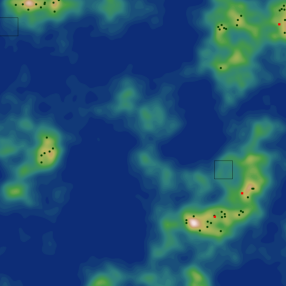
\includegraphics[interpolate=true,width=0.953333in,height=0.953333in]{terrain-img2.png}}%
\end{pgfscope}%
\begin{pgfscope}%
\pgfsetrectcap%
\pgfsetmiterjoin%
\pgfsetlinewidth{0.803000pt}%
\definecolor{currentstroke}{rgb}{0.000000,0.000000,0.000000}%
\pgfsetstrokecolor{currentstroke}%
\pgfsetdash{}{0pt}%
\pgfpathmoveto{\pgfqpoint{4.129803in}{2.771004in}}%
\pgfpathlineto{\pgfqpoint{4.129803in}{3.722147in}}%
\pgfusepath{stroke}%
\end{pgfscope}%
\begin{pgfscope}%
\pgfsetrectcap%
\pgfsetmiterjoin%
\pgfsetlinewidth{0.803000pt}%
\definecolor{currentstroke}{rgb}{0.000000,0.000000,0.000000}%
\pgfsetstrokecolor{currentstroke}%
\pgfsetdash{}{0pt}%
\pgfpathmoveto{\pgfqpoint{5.080946in}{2.771004in}}%
\pgfpathlineto{\pgfqpoint{5.080946in}{3.722147in}}%
\pgfusepath{stroke}%
\end{pgfscope}%
\begin{pgfscope}%
\pgfsetrectcap%
\pgfsetmiterjoin%
\pgfsetlinewidth{0.803000pt}%
\definecolor{currentstroke}{rgb}{0.000000,0.000000,0.000000}%
\pgfsetstrokecolor{currentstroke}%
\pgfsetdash{}{0pt}%
\pgfpathmoveto{\pgfqpoint{4.129803in}{2.771004in}}%
\pgfpathlineto{\pgfqpoint{5.080946in}{2.771004in}}%
\pgfusepath{stroke}%
\end{pgfscope}%
\begin{pgfscope}%
\pgfsetrectcap%
\pgfsetmiterjoin%
\pgfsetlinewidth{0.803000pt}%
\definecolor{currentstroke}{rgb}{0.000000,0.000000,0.000000}%
\pgfsetstrokecolor{currentstroke}%
\pgfsetdash{}{0pt}%
\pgfpathmoveto{\pgfqpoint{4.129803in}{3.722147in}}%
\pgfpathlineto{\pgfqpoint{5.080946in}{3.722147in}}%
\pgfusepath{stroke}%
\end{pgfscope}%
\begin{pgfscope}%
\pgfsetbuttcap%
\pgfsetmiterjoin%
\definecolor{currentfill}{rgb}{1.000000,1.000000,1.000000}%
\pgfsetfillcolor{currentfill}%
\pgfsetlinewidth{0.000000pt}%
\definecolor{currentstroke}{rgb}{0.000000,0.000000,0.000000}%
\pgfsetstrokecolor{currentstroke}%
\pgfsetstrokeopacity{0.000000}%
\pgfsetdash{}{0pt}%
\pgfpathmoveto{\pgfqpoint{4.129803in}{1.620319in}}%
\pgfpathlineto{\pgfqpoint{5.080946in}{1.620319in}}%
\pgfpathlineto{\pgfqpoint{5.080946in}{2.571462in}}%
\pgfpathlineto{\pgfqpoint{4.129803in}{2.571462in}}%
\pgfpathlineto{\pgfqpoint{4.129803in}{1.620319in}}%
\pgfpathclose%
\pgfusepath{fill}%
\end{pgfscope}%
\begin{pgfscope}%
\pgfpathrectangle{\pgfqpoint{4.129803in}{1.620319in}}{\pgfqpoint{0.951143in}{0.951143in}}%
\pgfusepath{clip}%
\pgfsys@transformshift{4.129803in}{1.620319in}%
\pgftext[left,bottom]{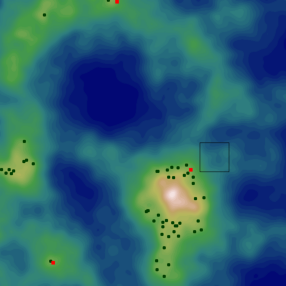
\includegraphics[interpolate=true,width=0.953333in,height=0.953333in]{terrain-img3.png}}%
\end{pgfscope}%
\begin{pgfscope}%
\pgfsetrectcap%
\pgfsetmiterjoin%
\pgfsetlinewidth{0.803000pt}%
\definecolor{currentstroke}{rgb}{0.000000,0.000000,0.000000}%
\pgfsetstrokecolor{currentstroke}%
\pgfsetdash{}{0pt}%
\pgfpathmoveto{\pgfqpoint{4.129803in}{1.620319in}}%
\pgfpathlineto{\pgfqpoint{4.129803in}{2.571462in}}%
\pgfusepath{stroke}%
\end{pgfscope}%
\begin{pgfscope}%
\pgfsetrectcap%
\pgfsetmiterjoin%
\pgfsetlinewidth{0.803000pt}%
\definecolor{currentstroke}{rgb}{0.000000,0.000000,0.000000}%
\pgfsetstrokecolor{currentstroke}%
\pgfsetdash{}{0pt}%
\pgfpathmoveto{\pgfqpoint{5.080946in}{1.620319in}}%
\pgfpathlineto{\pgfqpoint{5.080946in}{2.571462in}}%
\pgfusepath{stroke}%
\end{pgfscope}%
\begin{pgfscope}%
\pgfsetrectcap%
\pgfsetmiterjoin%
\pgfsetlinewidth{0.803000pt}%
\definecolor{currentstroke}{rgb}{0.000000,0.000000,0.000000}%
\pgfsetstrokecolor{currentstroke}%
\pgfsetdash{}{0pt}%
\pgfpathmoveto{\pgfqpoint{4.129803in}{1.620319in}}%
\pgfpathlineto{\pgfqpoint{5.080946in}{1.620319in}}%
\pgfusepath{stroke}%
\end{pgfscope}%
\begin{pgfscope}%
\pgfsetrectcap%
\pgfsetmiterjoin%
\pgfsetlinewidth{0.803000pt}%
\definecolor{currentstroke}{rgb}{0.000000,0.000000,0.000000}%
\pgfsetstrokecolor{currentstroke}%
\pgfsetdash{}{0pt}%
\pgfpathmoveto{\pgfqpoint{4.129803in}{2.571462in}}%
\pgfpathlineto{\pgfqpoint{5.080946in}{2.571462in}}%
\pgfusepath{stroke}%
\end{pgfscope}%
\begin{pgfscope}%
\pgfsetbuttcap%
\pgfsetmiterjoin%
\definecolor{currentfill}{rgb}{1.000000,1.000000,1.000000}%
\pgfsetfillcolor{currentfill}%
\pgfsetlinewidth{0.000000pt}%
\definecolor{currentstroke}{rgb}{0.000000,0.000000,0.000000}%
\pgfsetstrokecolor{currentstroke}%
\pgfsetstrokeopacity{0.000000}%
\pgfsetdash{}{0pt}%
\pgfpathmoveto{\pgfqpoint{4.129803in}{0.469634in}}%
\pgfpathlineto{\pgfqpoint{5.080946in}{0.469634in}}%
\pgfpathlineto{\pgfqpoint{5.080946in}{1.420777in}}%
\pgfpathlineto{\pgfqpoint{4.129803in}{1.420777in}}%
\pgfpathlineto{\pgfqpoint{4.129803in}{0.469634in}}%
\pgfpathclose%
\pgfusepath{fill}%
\end{pgfscope}%
\begin{pgfscope}%
\pgfpathrectangle{\pgfqpoint{4.129803in}{0.469634in}}{\pgfqpoint{0.951143in}{0.951143in}}%
\pgfusepath{clip}%
\pgfsys@transformshift{4.129803in}{0.469634in}%
\pgftext[left,bottom]{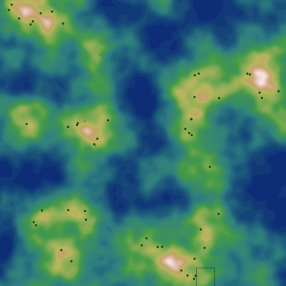
\includegraphics[interpolate=true,width=0.953333in,height=0.953333in]{terrain-img4.png}}%
\end{pgfscope}%
\begin{pgfscope}%
\pgfsetrectcap%
\pgfsetmiterjoin%
\pgfsetlinewidth{0.803000pt}%
\definecolor{currentstroke}{rgb}{0.000000,0.000000,0.000000}%
\pgfsetstrokecolor{currentstroke}%
\pgfsetdash{}{0pt}%
\pgfpathmoveto{\pgfqpoint{4.129803in}{0.469634in}}%
\pgfpathlineto{\pgfqpoint{4.129803in}{1.420777in}}%
\pgfusepath{stroke}%
\end{pgfscope}%
\begin{pgfscope}%
\pgfsetrectcap%
\pgfsetmiterjoin%
\pgfsetlinewidth{0.803000pt}%
\definecolor{currentstroke}{rgb}{0.000000,0.000000,0.000000}%
\pgfsetstrokecolor{currentstroke}%
\pgfsetdash{}{0pt}%
\pgfpathmoveto{\pgfqpoint{5.080946in}{0.469634in}}%
\pgfpathlineto{\pgfqpoint{5.080946in}{1.420777in}}%
\pgfusepath{stroke}%
\end{pgfscope}%
\begin{pgfscope}%
\pgfsetrectcap%
\pgfsetmiterjoin%
\pgfsetlinewidth{0.803000pt}%
\definecolor{currentstroke}{rgb}{0.000000,0.000000,0.000000}%
\pgfsetstrokecolor{currentstroke}%
\pgfsetdash{}{0pt}%
\pgfpathmoveto{\pgfqpoint{4.129803in}{0.469634in}}%
\pgfpathlineto{\pgfqpoint{5.080946in}{0.469634in}}%
\pgfusepath{stroke}%
\end{pgfscope}%
\begin{pgfscope}%
\pgfsetrectcap%
\pgfsetmiterjoin%
\pgfsetlinewidth{0.803000pt}%
\definecolor{currentstroke}{rgb}{0.000000,0.000000,0.000000}%
\pgfsetstrokecolor{currentstroke}%
\pgfsetdash{}{0pt}%
\pgfpathmoveto{\pgfqpoint{4.129803in}{1.420777in}}%
\pgfpathlineto{\pgfqpoint{5.080946in}{1.420777in}}%
\pgfusepath{stroke}%
\end{pgfscope}%
\end{pgfpicture}%
\makeatother%
\endgroup%

    \label{fig:terrain}
    %\vspace*{-1cm}
    \caption{Second environment. Terrain seen from above with ocean, }
\end{figure}

% environment 3: hard, realistic
The third environment is a three-dimensional version of the second one.
% 3D, or photos


% we discretize the problem
% should still apply to arbitrarily many dimensions
% assuming the existence of a suitable feature extractor

\section{Baseline}
\label{sec:baseline}

\section{Approach}
\label{sec:approach}

% should we rescale to 84x84 instead?

% https://www.reddit.com/r/reinforcementlearning/comments/ogwct6/how_to_deal_with_catastrophic_forgetting/
% hopefully reward normalization fixes it
% someone here does not recommend to clip value loss 

% https://arxiv.org/pdf/2006.05990.pdf
% cite this one...

% trade-off between end-to-end with RNN and modular system with explicit components, like memory.

% save latent representation of map?
% As in "Cognitive Mapping and Planning for Visual Navigation"

% self-supervised pretraining?
% https://arxiv.org/pdf/2003.14323.pdf

We postulate that an effective searcher should be able to:

\begin{itemize}
    \item Search the scene exhaustively, while avoiding visiting the same location multiple times.
    \item Learn a probability distribution of targets and its correlation with the appearance of the scene.
    \item Remember the appearance of previously visited areas in order to prioritize where to go next.
\end{itemize}

The agent is trained with reinforcement learning using Proximal Policy Optimization with function approximation using neural networks. 

% section 17.4 in sutton is good!

% https://xbpeng.github.io/projects/DeepMimic/index.html

% reward shaping: change reward signal as agent progresses
% could also shape the environment itself, make it more and more difficult
% each modification should be made so that the agent frequently receives reward with its current policy
% this is what we do when we train animals! ie give treats to dogs
% why isn't this working...

% reward normalization: 
% reward clipping: done in "playing atari with deep reinforcement learning": they state that since the scale of scores varies from game to game they fix all positive rewards to be one and negative to be -1. 0 rewards are left unchanged. this limits the scale of the error derivatives and makes it easier to use the same learning rate across multiple games. could also affect agent's performance as it cannot distinguish between rewards of different magnitudes.
% could be important for us if the number of targets and the reward varies a lot

% "explicit episodic (semantic) memory"
% visible region, visited regions
% other semantic information if available
% feature extraction with convolutions
% split the scene into discrete grid
% C channels with different features
% can even be applied to dynamic scenes with a last-seen mask

% could be multiple channels for view as well
% maybe call them "global" and "local"

\subsection{Architecture}

% resnets?
% https://efficientdl.com/how-to-train-a-resnet-efficiently/

% should use a constant network architecture

The architecture of the neural network is presented in Figure X.

The network is split into three main section: the feature extraction, the shared network, and the policy and value heads.

In order to be able to use the same extractor for all environments we resize the RGB image to \(64 \times 64\) pixels.

% Actor critic

% Feature extraction
% Shared Network
% Policy Head
% Value Head

% we should clearly explain the thought process
% connect back to local search problems
% we need a good feature extraction
% and then something for a belief state
% finally, what is the idea behind policy and value (should be in theory instead)

% we could give some pseudocode here

\section{Experiments}
\label{sec:experiments}

The first environment was used to determine a good observation space.
By just observing the current window, the agent can never learn a suitable policy to solve the problem.
This is because it cannot distinguish between equal windows at different locations.
Experiments are run with several additional observation types: window position, ...
Results of these experiments are presented for this environment only.

The agent was trained using the algorithm described in Section \ref{sec:approach} for 100 million time steps in all three environments using PPO, PPG and A2C.
Hyperparameters are tuned with random search separately for each environment.
For all experiments, the average return per episode is reported together with the theoretically optimal reward (obtained with an optimal path).
The agent was trained and tested on the full distribution of environments.

With the best performing algorithm we compare three different reward signals.
One gives a constant time penalty of -1 to incentivize finding the target quickly.
The second gives a constant time penalty of -2 and an exploration bonus of +1 when a new view is reached.
The third gives a reward of +1 for moving closer to the target and a penalty of -1 otherwise, as in \cite{caicedo_active_2015}.

Additionally, experiments to eveluate the generalization capability of the agent were conducted.
These were conducted on the procedurally generated terrain environment following the approach suggested in ~\cite{procgen}.
During training, the seed pool size was fixed to various sizes to limit the training set size.
The agent was trained for varying number of timesteps and then tested on the full distribution of environments.
This way, we can get a sense of how much data and simulation is required to use the approach for real-world tasks.

All experiments are conducted on an Intel Core i9-10900X CPU and an NVIDIA GeForce RTX 2080 Ti GPU.

For each experiment, we report the mean return and episode length over time during training.
We compare the approach to an exhaustive search and a human searcher with prior knowledge of the characteristics of the searched environments.
As per \cite{agarwal_rlliable_2022}, we report results across multiple seeds.

% could be the case that the supervised distance reward trains faster but leads to worse solutions that generalize worse
% should run experiments on this.


\section{Implementation}

The environment is implemented with Gym~\cite{brockman_gym_2016}, and the agent is implemented with PyTorch~\cite{paszke_pytorch_nodate}.
Proximal policy optimization was implemented following the official implementation by OpenAI.
Some necessary modifications were made to allow for recurrent policies.
% a little short...


% learning actions, recognition and localization simultaneously feels in itself interesting
% how do we interpret such a model? are there papers for visualizing reinforcement learning weights

% detailed
% replicability

% pre-study
% implementation
% evaluation

% discuss state representation
% need more than the image
% - either memory or position or both

% seed + 1000 levels training
% >= s + ... for test
% do the same as procgen

% also same configuration possibly?
% more parallel environments seem to lead to stable training (relatively slow increase in reward though...)

% would be nice to have a varying number of targets
% also a done action
% measure false positives, false negatives etc.
% good replacement for zoom?
% relates to visual search literature
% the current setup is also the most natural for a computer vision system
% foveated vision is not very reasonable


% select one algorithm and clearly motivate why!
% probably PPO, but why?


% time to find targets could be measured in terms of execution time, 
% and number of timesteps. this way, it could be easier to incorporate 
% visual attention if it is deemed reasonable.

% how do we handle appearance of targets:
% can an agent learn to recognize anything out of the ordinary?
% maybe not the focus, but just the search

% an interesting question is how large search windows we can handle
% could be an alternative to zoom
% a large search window presumably requires attention


% memory is needed for (a) remembering previous locations, and (b) integrating features over time


% PPO
% PPG
